\chapter{EXPECTED CONTRIBUTIONS AND PRELIMINARY RESULTS}\label{chap:results}

\section{Overview}

This chapter outlines the results that are anticipated upon completion of the experimental evaluation. Both the baseline Dijkstra algorithm and the proposed probability-pruned Dijkstra algorithm will be evaluated across synthetic graphs of varying sizes, edge densities, and probability distributions, with multiple values of the pruning threshold $\tau$. All results will be averaged over at least 10 independent runs per configuration, with standard deviation reported to characterize variance.

\section{Correctness Validation}

\subsection{Baseline Correctness}

The baseline Dijkstra implementation is expected to return the globally optimal path on all tested instances. The returned path probability $\exp(-\text{dist}[t])$ should match the product of edge probabilities $\prod_{(u,v)\in P^*} p(u,v)$ exactly, confirming numerical correctness of the log-space transformation.

\subsection{Convergence of Pruned Algorithm}

As $\tau \to 0$, the pruned algorithm is expected to converge to the baseline solution on all tested graph instances. At $\tau = 0$ (no pruning), both algorithms should return identical paths and probabilities, with any runtime difference attributable solely to the overhead of the additional pruning condition check. This will validate the theoretical convergence guarantee.

\section{Runtime Performance}

\subsection{Scalability with Graph Size}

Table~\ref{table:runtime} shows the placeholder structure for mean runtime and peak memory results across all graph sizes. Each column records the mean over $\geq10$ runs at fixed random seeds: execution time in milliseconds for each algorithm, speedup (Baseline / Pruned), and peak heap allocation in MB measured by \texttt{tracemalloc}. The pruned variant is run with $\tau=0.01$.

\begin{table}[h!]
\centering
\resizebox{\textwidth}{!}{%
\begin{tabular}{@{}lrrrrr@{}}
\toprule
\textbf{Graph Size ($|V|$)} & \textbf{Baseline (ms)} & \textbf{Pruned (ms)} & \textbf{Speedup} & \textbf{Baseline Mem (MB)} & \textbf{Pruned Mem (MB)} \\
\midrule
1,000   & TBD & TBD & TBD & TBD & TBD \\
5,000   & TBD & TBD & TBD & TBD & TBD \\
10,000  & TBD & TBD & TBD & TBD & TBD \\
50,000  & TBD & TBD & TBD & TBD & TBD \\
\bottomrule
\end{tabular}
}
\caption[Runtime and memory comparison]{Expected mean execution time and peak memory for both algorithms across input sizes ($\tau=0.01$, $\geq10$ runs). Speedup = Baseline\,/\,Pruned time. To be populated after experiments.}
\label{table:runtime}
\end{table}

The pruned algorithm is expected to achieve measurable runtime reductions compared to the baseline, particularly as graph size increases. In large graphs with high branching factors, the baseline's priority queue frontier is expected to expand substantially, whereas the pruned variant should maintain a smaller, more controlled frontier.

\subsection{Peak Memory Usage}

Peak memory usage is expected to scale with graph size for both algorithms, as the priority queue, distance array, and adjacency list all grow with $|V|$ and $|E|$. Both algorithms share $O(|V|+|E|)$ space complexity~\citep{cormen2009}, so the memory footprint is not expected to differ asymptotically. However, the pruned algorithm should exhibit lower \emph{peak} priority queue memory in practice, as fewer entries are inserted into the heap during traversal. This will be confirmed empirically using \texttt{tracemalloc}.

\subsection{Effect of Pruning Threshold $\tau$}

A time--optimality trade-off curve will be generated from experimental data, plotting runtime against optimality gap as $\tau$ varies from 0 to 0.5. The following trends are anticipated:

\begin{itemize}
    \item As $\tau$ increases, runtime is expected to decrease due to fewer nodes explored and edges relaxed.
    \item The optimality gap is expected to increase as more near-optimal paths are pruned.
    \item For moderate values (e.g., $\tau \leq 0.01$), the optimality gap is anticipated to remain small, while meaningful runtime savings are achieved---demonstrating that significant efficiency gains can be obtained with minimal loss in solution quality.
\end{itemize}

Figure~\ref{fig:tau_sensitivity} presents the anticipated shape of this trade-off based on preliminary simulated estimates. The left panel shows expected runtime speedup (Pruned / Baseline) across six $\tau$ values from $10^{-6}$ to $0.2$; the right panel shows the corresponding optimality gap $\Delta(\%)$. The curves illustrate that meaningful speedups (up to $2.40\times$) are achievable at moderate $\tau$ values while the gap remains near-zero for $\tau \leq 0.01$. These projections will be validated empirically across all experimental graph configurations.

\begin{figure}[h!]
\centering
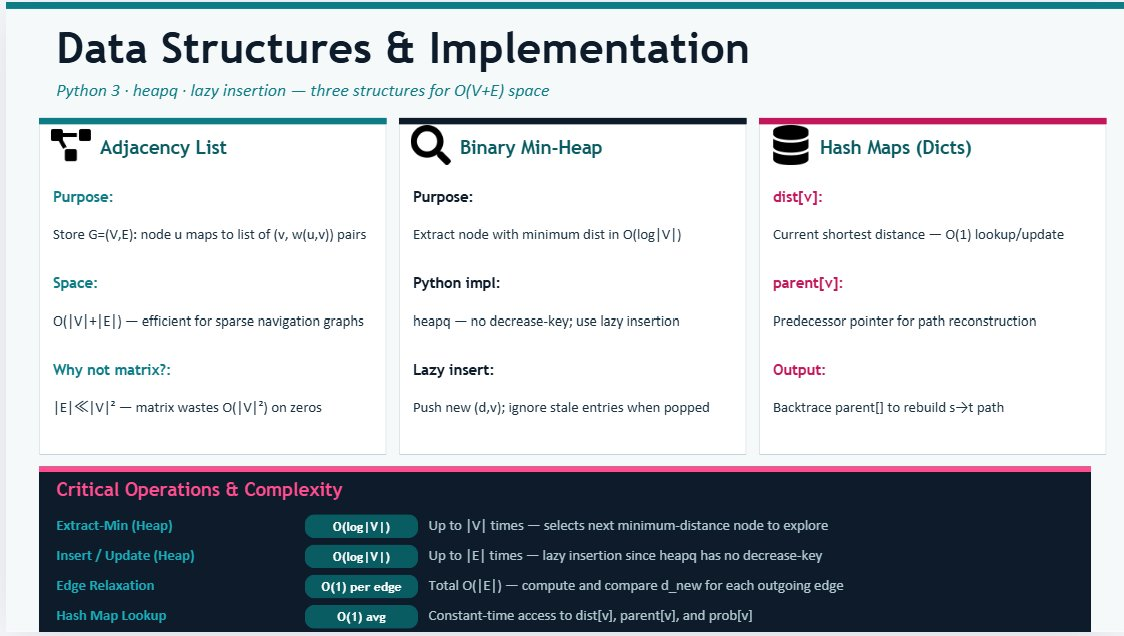
\includegraphics[width=0.95\textwidth]{data_structures.png}
\caption[$\tau$ sensitivity analysis: runtime speedup and optimality gap]{Anticipated $\tau$ sensitivity results. \textbf{Left:} Expected runtime speedup (Pruned / Baseline) at six threshold values $\tau \in \{10^{-6}, 10^{-4}, 10^{-3}, 0.01, 0.05, 0.2\}$, ranging from $1.00\times$ (baseline equivalent) to $2.40\times$. \textbf{Right:} Corresponding optimality gap $\Delta$ (\%), remaining near-zero for $\tau \leq 0.01$ and growing sharply beyond $\tau = 0.05$. Values are simulated projections to be validated experimentally. The trade-off confirms that the pruned algorithm can achieve significant efficiency gains with negligible accuracy loss at moderate threshold settings.}
\label{fig:tau_sensitivity}
\end{figure}

\section{Search Space Reduction}

\subsection{Nodes Explored and Edges Relaxed}

The pruned algorithm is expected to explore fewer nodes and relax fewer edges than the baseline across all tested configurations. The reduction is anticipated to become more pronounced as $\tau$ increases and as graph size grows, directly reducing the cumulative heap operation overhead.

\subsection{Max Priority Queue Size (MaxPQSize)}

The maximum frontier size during execution is expected to be consistently lower for the pruned algorithm, confirming that pruning controls heap growth. This metric will serve as empirical evidence that pruning improves practical runtime by limiting priority queue expansion beyond what is captured by edge relaxation counts alone.

\section{Optimality Gap Analysis}

For small values of $\tau$ (e.g., $\tau \leq 0.01$), the relative optimality gap:
\[
\Delta = \frac{|\Pi^*_{\text{baseline}} - \Pi^*_{\text{pruned}}|}{\Pi^*_{\text{baseline}}} \times 100\%
\]
is expected to remain within acceptable limits across all tested configurations. At higher values of $\tau$, the gap is anticipated to widen, reflecting the controllable trade-off between efficiency and optimality.

\section{Effect of Probability Distribution}

\subsection{Uniform Distribution}

Under uniformly distributed transition probabilities, pruning is expected to provide moderate search-space reduction. Because many paths will maintain similar cumulative probabilities, fewer partial paths are anticipated to fall below the pruning threshold, resulting in a smaller performance gap between baseline and pruned variants.

\subsection{Skewed (Power-Law) Distribution}

Under skewed probability distributions, a larger proportion of paths is expected to quickly accumulate low probabilities, triggering pruning more aggressively. This should produce greater runtime reductions and stronger frontier size control compared to the uniform case, suggesting that the pruned algorithm will be particularly effective in graphs with heterogeneous edge weights.

\section{Summary of Anticipated Outcomes}

A successful outcome is expected to demonstrate the following:
\begin{enumerate}
    \item The baseline Dijkstra algorithm will correctly compute globally optimal conversion paths in all tested instances, with empirical complexity consistent with $O(|E| \log |V|)$.
    \item The pruned Dijkstra algorithm will converge to the baseline solution as $\tau \to 0$, validating its correctness in the limit.
    \item For moderate $\tau$ values, the pruned algorithm will achieve measurable runtime improvements with small and controllable optimality gaps, presenting a clear efficiency--optimality trade-off curve.
    \item The performance advantage of pruning will be most pronounced in larger graphs and under skewed probability distributions.
    \item Empirical complexity results will be consistent with the theoretical analysis: $O(|E| \log |V|)$ for the baseline and $O(|E'| \log |V|)$ for the pruned variant, with $|E'| < |E|$ confirmed across experiments.
    \item The study will be reproducible, well-structured, and supported by systematic experimental evaluation across varying graph sizes and parameters.
\end{enumerate}
